\documentclass[11pt]{beamer}
\usepackage[english]{babel}
\usepackage{graphicx}
\usepackage{color}
\usepackage{amsmath,amssymb}
\usetheme{madrid}
\usecolortheme{default}
\title{\textit{THREE CURVES}}
\subtitle{\textit{20411885}}
\author{Junfeng Zhu}
\institute{UNNC}
\date{\today}

\begin{document}
\begin{frame}\label{TP}
\titlepage
\end{frame}

\begin{frame}\frametitle{TABLE OF CONTENT}\label{TOC}
\tableofcontents
\end{frame}

\section{THREE FUNCTION}
\begin{frame}\frametitle{THREE FUNCTION}\label{TF}
\begin{columns}
\column{0.5\textwidth}

\begin{eqnarray*} 
\begin{cases}

\textcolor{blue}{y =  e^{x^3-1}}\\
\textcolor{green}{z =  2x\*e^{x^3-1}}\\
w =  x\*\sin(x)-1

\end{cases}
\end{eqnarray*}

\pause

\column{0.5\textwidth}
\begin{figure}
\centering
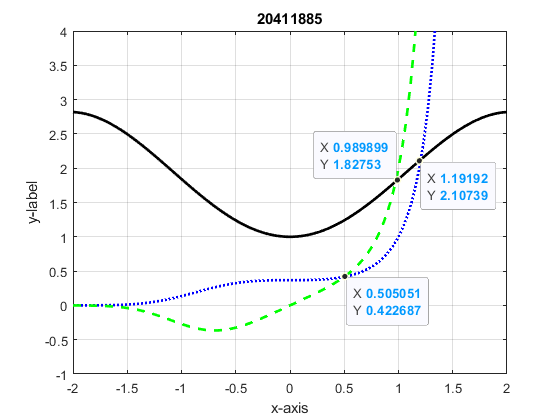
\includegraphics[scale=0.45]{threecurves}
\caption{\textit{THREE CURVES}}
\end{figure}
\end{columns}
\end{frame}

\section{OBSERVATIONS}
\begin{frame}\frametitle{OBSERVATIONS}\label{O}

\begin{table}[h]
\centering
\begin{tabular}{c|c|c|c}
Function&Intersection with $f$&Intersection with $g$&Intersection with $h$\\
\hline
\hline
$f(x)$&$-$&$(0.51,0.42)$&$(1.19,2.11)$\\
\hline
$g(x)$&$(0.51,0.42)$&$-$&$(0.99,1.83)$\\
\hline
$h(x)$&$(1.19,2.11)$&$(0.99,1.83)$&$-$\\
\hline

\end{tabular}
\caption{Table of observations}
\end{table}

\end{frame}
\section{SUMMARY}
\begin{frame}\frametitle{SUMMARY}

\hyperlink{TP}{\beamergotobutton{Back to Title}}\\
\hyperlink{TOC}{\beamergotobutton{Back to Table of Contents}}\\
\hyperlink{TF}{\beamergotobutton{Back to Three Functions}}\\
\hyperlink{O}{\beamergotobutton{Back to Observations}}

\end{frame}

\end{document}